% Created by tikzDevice version 0.6.2-92-0ad2792 on 2013-03-04 10:17:46
% !TEX encoding = UTF-8 Unicode
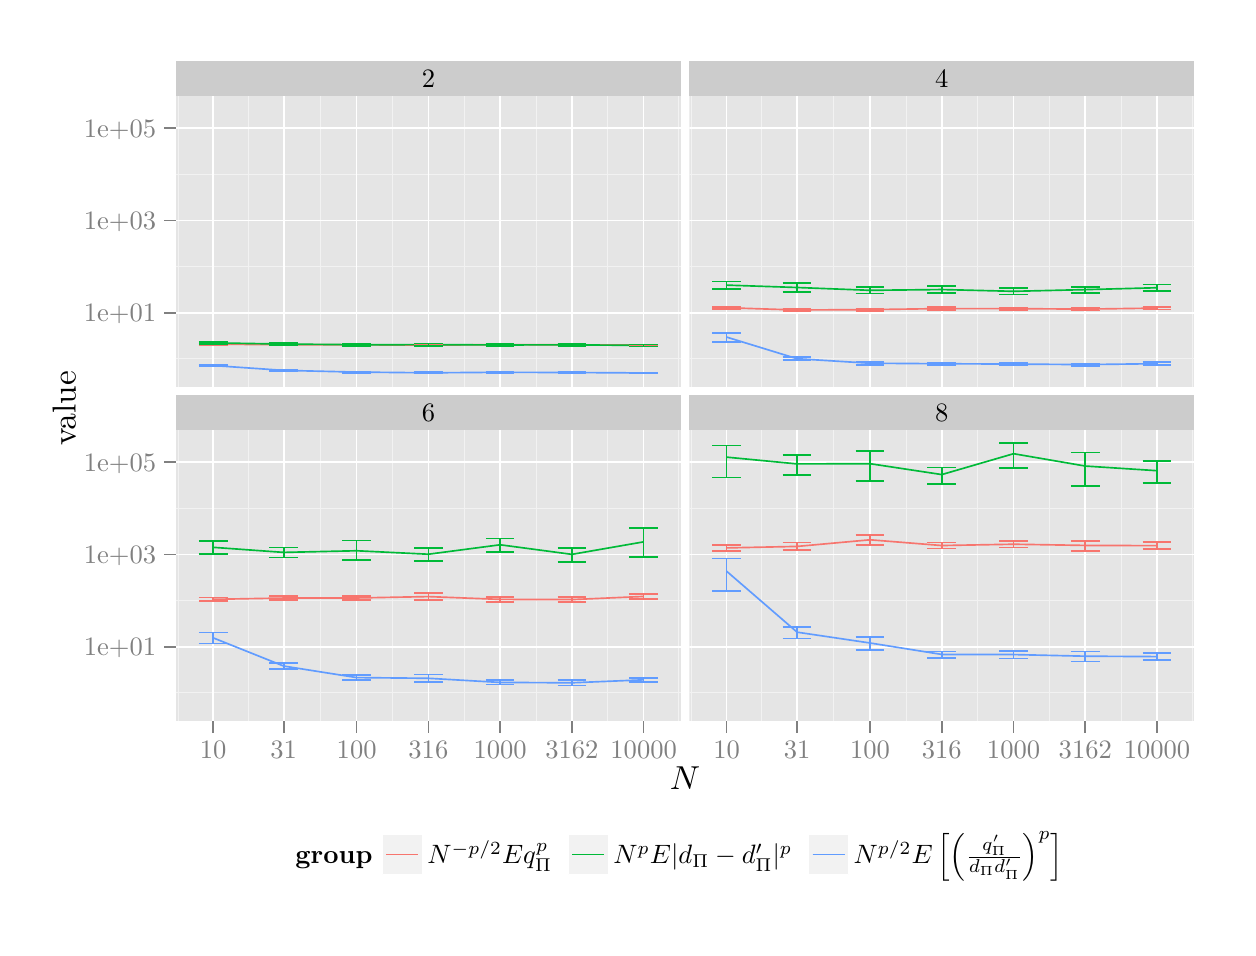
\begin{tikzpicture}[x=1pt,y=1pt]
\definecolor[named]{fillColor}{rgb}{1.00,1.00,1.00}
\path[use as bounding box,fill=fillColor,fill opacity=0.00] (0,0) rectangle (433.62,325.21);
\begin{scope}
\path[clip] (  0.00,  0.00) rectangle (433.62,325.21);
\definecolor[named]{drawColor}{rgb}{1.00,1.00,1.00}
\definecolor[named]{fillColor}{rgb}{1.00,1.00,1.00}

\path[draw=drawColor,line width= 0.6pt,line join=round,line cap=round,fill=fillColor] (  0.00,  0.00) rectangle (433.62,325.21);
\end{scope}
\begin{scope}
\path[clip] ( 53.55,195.47) rectangle (236.06,300.54);
\definecolor[named]{fillColor}{rgb}{0.90,0.90,0.90}

\path[fill=fillColor] ( 53.55,195.47) rectangle (236.06,300.54);
\definecolor[named]{drawColor}{rgb}{0.95,0.95,0.95}

\path[draw=drawColor,line width= 0.3pt,line join=round] ( 53.55,205.55) --
	(236.06,205.55);

\path[draw=drawColor,line width= 0.3pt,line join=round] ( 53.55,238.90) --
	(236.06,238.90);

\path[draw=drawColor,line width= 0.3pt,line join=round] ( 53.55,272.26) --
	(236.06,272.26);

\path[draw=drawColor,line width= 0.3pt,line join=round] ( 54.29,195.47) --
	( 54.29,300.54);

\path[draw=drawColor,line width= 0.3pt,line join=round] ( 79.77,195.47) --
	( 79.77,300.54);

\path[draw=drawColor,line width= 0.3pt,line join=round] (105.69,195.47) --
	(105.69,300.54);

\path[draw=drawColor,line width= 0.3pt,line join=round] (131.83,195.47) --
	(131.83,300.54);

\path[draw=drawColor,line width= 0.3pt,line join=round] (157.76,195.47) --
	(157.76,300.54);

\path[draw=drawColor,line width= 0.3pt,line join=round] (183.69,195.47) --
	(183.69,300.54);

\path[draw=drawColor,line width= 0.3pt,line join=round] (209.61,195.47) --
	(209.61,300.54);

\path[draw=drawColor,line width= 0.3pt,line join=round] (235.31,195.47) --
	(235.31,300.54);
\definecolor[named]{drawColor}{rgb}{1.00,1.00,1.00}

\path[draw=drawColor,line width= 0.6pt,line join=round] ( 53.55,222.22) --
	(236.06,222.22);

\path[draw=drawColor,line width= 0.6pt,line join=round] ( 53.55,255.58) --
	(236.06,255.58);

\path[draw=drawColor,line width= 0.6pt,line join=round] ( 53.55,288.94) --
	(236.06,288.94);

\path[draw=drawColor,line width= 0.6pt,line join=round] ( 67.03,195.47) --
	( 67.03,300.54);

\path[draw=drawColor,line width= 0.6pt,line join=round] ( 92.51,195.47) --
	( 92.51,300.54);

\path[draw=drawColor,line width= 0.6pt,line join=round] (118.88,195.47) --
	(118.88,300.54);

\path[draw=drawColor,line width= 0.6pt,line join=round] (144.79,195.47) --
	(144.79,300.54);

\path[draw=drawColor,line width= 0.6pt,line join=round] (170.73,195.47) --
	(170.73,300.54);

\path[draw=drawColor,line width= 0.6pt,line join=round] (196.65,195.47) --
	(196.65,300.54);

\path[draw=drawColor,line width= 0.6pt,line join=round] (222.58,195.47) --
	(222.58,300.54);
\definecolor[named]{drawColor}{rgb}{0.97,0.46,0.43}

\path[draw=drawColor,line width= 0.6pt,line join=round] ( 67.03,210.83) --
	( 92.51,210.65) --
	(118.88,210.61) --
	(144.79,210.48) --
	(170.73,210.68) --
	(196.65,210.63) --
	(222.58,210.49);
\definecolor[named]{drawColor}{rgb}{0.00,0.73,0.22}

\path[draw=drawColor,line width= 0.6pt,line join=round] ( 67.03,211.31) --
	( 92.51,210.88) --
	(118.88,210.64) --
	(144.79,210.67) --
	(170.73,210.56) --
	(196.65,210.59) --
	(222.58,210.39);
\definecolor[named]{drawColor}{rgb}{0.38,0.61,1.00}

\path[draw=drawColor,line width= 0.6pt,line join=round] ( 67.03,203.12) --
	( 92.51,201.37) --
	(118.88,200.75) --
	(144.79,200.49) --
	(170.73,200.68) --
	(196.65,200.59) --
	(222.58,200.45);
\definecolor[named]{drawColor}{rgb}{0.97,0.46,0.43}

\path[draw=drawColor,line width= 0.6pt,line join=round] ( 61.85,211.01) --
	( 72.22,211.01);

\path[draw=drawColor,line width= 0.6pt,line join=round] ( 67.03,211.01) --
	( 67.03,210.64);

\path[draw=drawColor,line width= 0.6pt,line join=round] ( 61.85,210.64) --
	( 72.22,210.64);

\path[draw=drawColor,line width= 0.6pt,line join=round] ( 87.32,210.85) --
	( 97.69,210.85);

\path[draw=drawColor,line width= 0.6pt,line join=round] ( 92.51,210.85) --
	( 92.51,210.45);

\path[draw=drawColor,line width= 0.6pt,line join=round] ( 87.32,210.45) --
	( 97.69,210.45);

\path[draw=drawColor,line width= 0.6pt,line join=round] (113.69,210.80) --
	(124.06,210.80);

\path[draw=drawColor,line width= 0.6pt,line join=round] (118.88,210.80) --
	(118.88,210.41);

\path[draw=drawColor,line width= 0.6pt,line join=round] (113.69,210.41) --
	(124.06,210.41);

\path[draw=drawColor,line width= 0.6pt,line join=round] (139.60,210.68) --
	(149.97,210.68);

\path[draw=drawColor,line width= 0.6pt,line join=round] (144.79,210.68) --
	(144.79,210.27);

\path[draw=drawColor,line width= 0.6pt,line join=round] (139.60,210.27) --
	(149.97,210.27);

\path[draw=drawColor,line width= 0.6pt,line join=round] (165.54,210.87) --
	(175.91,210.87);

\path[draw=drawColor,line width= 0.6pt,line join=round] (170.73,210.87) --
	(170.73,210.48);

\path[draw=drawColor,line width= 0.6pt,line join=round] (165.54,210.48) --
	(175.91,210.48);

\path[draw=drawColor,line width= 0.6pt,line join=round] (191.47,210.82) --
	(201.83,210.82);

\path[draw=drawColor,line width= 0.6pt,line join=round] (196.65,210.82) --
	(196.65,210.42);

\path[draw=drawColor,line width= 0.6pt,line join=round] (191.47,210.42) --
	(201.83,210.42);

\path[draw=drawColor,line width= 0.6pt,line join=round] (217.39,210.69) --
	(227.76,210.69);

\path[draw=drawColor,line width= 0.6pt,line join=round] (222.58,210.69) --
	(222.58,210.29);

\path[draw=drawColor,line width= 0.6pt,line join=round] (217.39,210.29) --
	(227.76,210.29);
\definecolor[named]{drawColor}{rgb}{0.00,0.73,0.22}

\path[draw=drawColor,line width= 0.6pt,line join=round] ( 61.85,211.65) --
	( 72.22,211.65);

\path[draw=drawColor,line width= 0.6pt,line join=round] ( 67.03,211.65) --
	( 67.03,210.96);

\path[draw=drawColor,line width= 0.6pt,line join=round] ( 61.85,210.96) --
	( 72.22,210.96);

\path[draw=drawColor,line width= 0.6pt,line join=round] ( 87.32,211.25) --
	( 97.69,211.25);

\path[draw=drawColor,line width= 0.6pt,line join=round] ( 92.51,211.25) --
	( 92.51,210.53);

\path[draw=drawColor,line width= 0.6pt,line join=round] ( 87.32,210.53) --
	( 97.69,210.53);

\path[draw=drawColor,line width= 0.6pt,line join=round] (113.69,211.01) --
	(124.06,211.01);

\path[draw=drawColor,line width= 0.6pt,line join=round] (118.88,211.01) --
	(118.88,210.29);

\path[draw=drawColor,line width= 0.6pt,line join=round] (113.69,210.29) --
	(124.06,210.29);

\path[draw=drawColor,line width= 0.6pt,line join=round] (139.60,211.06) --
	(149.97,211.06);

\path[draw=drawColor,line width= 0.6pt,line join=round] (144.79,211.06) --
	(144.79,210.28);

\path[draw=drawColor,line width= 0.6pt,line join=round] (139.60,210.28) --
	(149.97,210.28);

\path[draw=drawColor,line width= 0.6pt,line join=round] (165.54,210.98) --
	(175.91,210.98);

\path[draw=drawColor,line width= 0.6pt,line join=round] (170.73,210.98) --
	(170.73,210.19);

\path[draw=drawColor,line width= 0.6pt,line join=round] (165.54,210.19) --
	(175.91,210.19);

\path[draw=drawColor,line width= 0.6pt,line join=round] (191.47,210.96) --
	(201.83,210.96);

\path[draw=drawColor,line width= 0.6pt,line join=round] (196.65,210.96) --
	(196.65,210.23);

\path[draw=drawColor,line width= 0.6pt,line join=round] (191.47,210.23) --
	(201.83,210.23);

\path[draw=drawColor,line width= 0.6pt,line join=round] (217.39,210.75) --
	(227.76,210.75);

\path[draw=drawColor,line width= 0.6pt,line join=round] (222.58,210.75) --
	(222.58,209.99);

\path[draw=drawColor,line width= 0.6pt,line join=round] (217.39,209.99) --
	(227.76,209.99);
\definecolor[named]{drawColor}{rgb}{0.38,0.61,1.00}

\path[draw=drawColor,line width= 0.6pt,line join=round] ( 61.85,203.39) --
	( 72.22,203.39);

\path[draw=drawColor,line width= 0.6pt,line join=round] ( 67.03,203.39) --
	( 67.03,202.84);

\path[draw=drawColor,line width= 0.6pt,line join=round] ( 61.85,202.84) --
	( 72.22,202.84);

\path[draw=drawColor,line width= 0.6pt,line join=round] ( 87.32,201.61) --
	( 97.69,201.61);

\path[draw=drawColor,line width= 0.6pt,line join=round] ( 92.51,201.61) --
	( 92.51,201.15);

\path[draw=drawColor,line width= 0.6pt,line join=round] ( 87.32,201.15) --
	( 97.69,201.15);

\path[draw=drawColor,line width= 0.6pt,line join=round] (113.69,200.95) --
	(124.06,200.95);

\path[draw=drawColor,line width= 0.6pt,line join=round] (118.88,200.95) --
	(118.88,200.54);

\path[draw=drawColor,line width= 0.6pt,line join=round] (113.69,200.54) --
	(124.06,200.54);

\path[draw=drawColor,line width= 0.6pt,line join=round] (139.60,200.68) --
	(149.97,200.68);

\path[draw=drawColor,line width= 0.6pt,line join=round] (144.79,200.68) --
	(144.79,200.29);

\path[draw=drawColor,line width= 0.6pt,line join=round] (139.60,200.29) --
	(149.97,200.29);

\path[draw=drawColor,line width= 0.6pt,line join=round] (165.54,200.87) --
	(175.91,200.87);

\path[draw=drawColor,line width= 0.6pt,line join=round] (170.73,200.87) --
	(170.73,200.48);

\path[draw=drawColor,line width= 0.6pt,line join=round] (165.54,200.48) --
	(175.91,200.48);

\path[draw=drawColor,line width= 0.6pt,line join=round] (191.47,200.80) --
	(201.83,200.80);

\path[draw=drawColor,line width= 0.6pt,line join=round] (196.65,200.80) --
	(196.65,200.39);

\path[draw=drawColor,line width= 0.6pt,line join=round] (191.47,200.39) --
	(201.83,200.39);

\path[draw=drawColor,line width= 0.6pt,line join=round] (217.39,200.64) --
	(227.76,200.64);

\path[draw=drawColor,line width= 0.6pt,line join=round] (222.58,200.64) --
	(222.58,200.25);

\path[draw=drawColor,line width= 0.6pt,line join=round] (217.39,200.25) --
	(227.76,200.25);
\end{scope}
\begin{scope}
\path[clip] (239.07,195.47) rectangle (421.58,300.54);
\definecolor[named]{fillColor}{rgb}{0.90,0.90,0.90}

\path[fill=fillColor] (239.07,195.47) rectangle (421.57,300.54);
\definecolor[named]{drawColor}{rgb}{0.95,0.95,0.95}

\path[draw=drawColor,line width= 0.3pt,line join=round] (239.07,205.55) --
	(421.58,205.55);

\path[draw=drawColor,line width= 0.3pt,line join=round] (239.07,238.90) --
	(421.58,238.90);

\path[draw=drawColor,line width= 0.3pt,line join=round] (239.07,272.26) --
	(421.58,272.26);

\path[draw=drawColor,line width= 0.3pt,line join=round] (239.81,195.47) --
	(239.81,300.54);

\path[draw=drawColor,line width= 0.3pt,line join=round] (265.29,195.47) --
	(265.29,300.54);

\path[draw=drawColor,line width= 0.3pt,line join=round] (291.21,195.47) --
	(291.21,300.54);

\path[draw=drawColor,line width= 0.3pt,line join=round] (317.35,195.47) --
	(317.35,300.54);

\path[draw=drawColor,line width= 0.3pt,line join=round] (343.28,195.47) --
	(343.28,300.54);

\path[draw=drawColor,line width= 0.3pt,line join=round] (369.21,195.47) --
	(369.21,300.54);

\path[draw=drawColor,line width= 0.3pt,line join=round] (395.13,195.47) --
	(395.13,300.54);

\path[draw=drawColor,line width= 0.3pt,line join=round] (420.83,195.47) --
	(420.83,300.54);
\definecolor[named]{drawColor}{rgb}{1.00,1.00,1.00}

\path[draw=drawColor,line width= 0.6pt,line join=round] (239.07,222.22) --
	(421.58,222.22);

\path[draw=drawColor,line width= 0.6pt,line join=round] (239.07,255.58) --
	(421.58,255.58);

\path[draw=drawColor,line width= 0.6pt,line join=round] (239.07,288.94) --
	(421.58,288.94);

\path[draw=drawColor,line width= 0.6pt,line join=round] (252.55,195.47) --
	(252.55,300.54);

\path[draw=drawColor,line width= 0.6pt,line join=round] (278.03,195.47) --
	(278.03,300.54);

\path[draw=drawColor,line width= 0.6pt,line join=round] (304.40,195.47) --
	(304.40,300.54);

\path[draw=drawColor,line width= 0.6pt,line join=round] (330.31,195.47) --
	(330.31,300.54);

\path[draw=drawColor,line width= 0.6pt,line join=round] (356.25,195.47) --
	(356.25,300.54);

\path[draw=drawColor,line width= 0.6pt,line join=round] (382.17,195.47) --
	(382.17,300.54);

\path[draw=drawColor,line width= 0.6pt,line join=round] (408.09,195.47) --
	(408.09,300.54);
\definecolor[named]{drawColor}{rgb}{0.97,0.46,0.43}

\path[draw=drawColor,line width= 0.6pt,line join=round] (252.55,224.00) --
	(278.03,223.19) --
	(304.40,223.33) --
	(330.31,223.70) --
	(356.25,223.68) --
	(382.17,223.51) --
	(408.09,223.87);
\definecolor[named]{drawColor}{rgb}{0.00,0.73,0.22}

\path[draw=drawColor,line width= 0.6pt,line join=round] (252.55,232.18) --
	(278.03,231.32) --
	(304.40,230.30) --
	(330.31,230.58) --
	(356.25,229.94) --
	(382.17,230.55) --
	(408.09,231.23);
\definecolor[named]{drawColor}{rgb}{0.38,0.61,1.00}

\path[draw=drawColor,line width= 0.6pt,line join=round] (252.55,213.40) --
	(278.03,205.58) --
	(304.40,203.95) --
	(330.31,203.77) --
	(356.25,203.65) --
	(382.17,203.46) --
	(408.09,203.79);
\definecolor[named]{drawColor}{rgb}{0.97,0.46,0.43}

\path[draw=drawColor,line width= 0.6pt,line join=round] (247.36,224.39) --
	(257.73,224.39);

\path[draw=drawColor,line width= 0.6pt,line join=round] (252.55,224.39) --
	(252.55,223.60);

\path[draw=drawColor,line width= 0.6pt,line join=round] (247.36,223.60) --
	(257.73,223.60);

\path[draw=drawColor,line width= 0.6pt,line join=round] (272.84,223.58) --
	(283.21,223.58);

\path[draw=drawColor,line width= 0.6pt,line join=round] (278.03,223.58) --
	(278.03,222.78);

\path[draw=drawColor,line width= 0.6pt,line join=round] (272.84,222.78) --
	(283.21,222.78);

\path[draw=drawColor,line width= 0.6pt,line join=round] (299.21,223.79) --
	(309.58,223.79);

\path[draw=drawColor,line width= 0.6pt,line join=round] (304.40,223.79) --
	(304.40,222.82);

\path[draw=drawColor,line width= 0.6pt,line join=round] (299.21,222.82) --
	(309.58,222.82);

\path[draw=drawColor,line width= 0.6pt,line join=round] (325.12,224.18) --
	(335.49,224.18);

\path[draw=drawColor,line width= 0.6pt,line join=round] (330.31,224.18) --
	(330.31,223.27);

\path[draw=drawColor,line width= 0.6pt,line join=round] (325.12,223.27) --
	(335.49,223.27);

\path[draw=drawColor,line width= 0.6pt,line join=round] (351.06,224.07) --
	(361.43,224.07);

\path[draw=drawColor,line width= 0.6pt,line join=round] (356.25,224.07) --
	(356.25,223.27);

\path[draw=drawColor,line width= 0.6pt,line join=round] (351.06,223.27) --
	(361.43,223.27);

\path[draw=drawColor,line width= 0.6pt,line join=round] (376.98,223.94) --
	(387.35,223.94);

\path[draw=drawColor,line width= 0.6pt,line join=round] (382.17,223.94) --
	(382.17,223.04);

\path[draw=drawColor,line width= 0.6pt,line join=round] (376.98,223.04) --
	(387.35,223.04);

\path[draw=drawColor,line width= 0.6pt,line join=round] (402.91,224.35) --
	(413.28,224.35);

\path[draw=drawColor,line width= 0.6pt,line join=round] (408.09,224.35) --
	(408.09,223.37);

\path[draw=drawColor,line width= 0.6pt,line join=round] (402.91,223.37) --
	(413.28,223.37);
\definecolor[named]{drawColor}{rgb}{0.00,0.73,0.22}

\path[draw=drawColor,line width= 0.6pt,line join=round] (247.36,233.48) --
	(257.73,233.48);

\path[draw=drawColor,line width= 0.6pt,line join=round] (252.55,233.48) --
	(252.55,230.83);

\path[draw=drawColor,line width= 0.6pt,line join=round] (247.36,230.83) --
	(257.73,230.83);

\path[draw=drawColor,line width= 0.6pt,line join=round] (272.84,232.93) --
	(283.21,232.93);

\path[draw=drawColor,line width= 0.6pt,line join=round] (278.03,232.93) --
	(278.03,229.73);

\path[draw=drawColor,line width= 0.6pt,line join=round] (272.84,229.73) --
	(283.21,229.73);

\path[draw=drawColor,line width= 0.6pt,line join=round] (299.21,231.38) --
	(309.58,231.38);

\path[draw=drawColor,line width= 0.6pt,line join=round] (304.40,231.38) --
	(304.40,229.17);

\path[draw=drawColor,line width= 0.6pt,line join=round] (299.21,229.17) --
	(309.58,229.17);

\path[draw=drawColor,line width= 0.6pt,line join=round] (325.12,231.92) --
	(335.49,231.92);

\path[draw=drawColor,line width= 0.6pt,line join=round] (330.31,231.92) --
	(330.31,229.26);

\path[draw=drawColor,line width= 0.6pt,line join=round] (325.12,229.26) --
	(335.49,229.26);

\path[draw=drawColor,line width= 0.6pt,line join=round] (351.06,231.17) --
	(361.43,231.17);

\path[draw=drawColor,line width= 0.6pt,line join=round] (356.25,231.17) --
	(356.25,228.79);

\path[draw=drawColor,line width= 0.6pt,line join=round] (351.06,228.79) --
	(361.43,228.79);

\path[draw=drawColor,line width= 0.6pt,line join=round] (376.98,231.58) --
	(387.35,231.58);

\path[draw=drawColor,line width= 0.6pt,line join=round] (382.17,231.58) --
	(382.17,229.45);

\path[draw=drawColor,line width= 0.6pt,line join=round] (376.98,229.45) --
	(387.35,229.45);

\path[draw=drawColor,line width= 0.6pt,line join=round] (402.91,232.36) --
	(413.28,232.36);

\path[draw=drawColor,line width= 0.6pt,line join=round] (408.09,232.36) --
	(408.09,230.04);

\path[draw=drawColor,line width= 0.6pt,line join=round] (402.91,230.04) --
	(413.28,230.04);
\definecolor[named]{drawColor}{rgb}{0.38,0.61,1.00}

\path[draw=drawColor,line width= 0.6pt,line join=round] (247.36,214.84) --
	(257.73,214.84);

\path[draw=drawColor,line width= 0.6pt,line join=round] (252.55,214.84) --
	(252.55,211.68);

\path[draw=drawColor,line width= 0.6pt,line join=round] (247.36,211.68) --
	(257.73,211.68);

\path[draw=drawColor,line width= 0.6pt,line join=round] (272.84,206.09) --
	(283.21,206.09);

\path[draw=drawColor,line width= 0.6pt,line join=round] (278.03,206.09) --
	(278.03,205.09);

\path[draw=drawColor,line width= 0.6pt,line join=round] (272.84,205.09) --
	(283.21,205.09);

\path[draw=drawColor,line width= 0.6pt,line join=round] (299.21,204.39) --
	(309.58,204.39);

\path[draw=drawColor,line width= 0.6pt,line join=round] (304.40,204.39) --
	(304.40,203.43);

\path[draw=drawColor,line width= 0.6pt,line join=round] (299.21,203.43) --
	(309.58,203.43);

\path[draw=drawColor,line width= 0.6pt,line join=round] (325.12,204.22) --
	(335.49,204.22);

\path[draw=drawColor,line width= 0.6pt,line join=round] (330.31,204.22) --
	(330.31,203.28);

\path[draw=drawColor,line width= 0.6pt,line join=round] (325.12,203.28) --
	(335.49,203.28);

\path[draw=drawColor,line width= 0.6pt,line join=round] (351.06,204.09) --
	(361.43,204.09);

\path[draw=drawColor,line width= 0.6pt,line join=round] (356.25,204.09) --
	(356.25,203.21);

\path[draw=drawColor,line width= 0.6pt,line join=round] (351.06,203.21) --
	(361.43,203.21);

\path[draw=drawColor,line width= 0.6pt,line join=round] (376.98,203.91) --
	(387.35,203.91);

\path[draw=drawColor,line width= 0.6pt,line join=round] (382.17,203.91) --
	(382.17,202.96);

\path[draw=drawColor,line width= 0.6pt,line join=round] (376.98,202.96) --
	(387.35,202.96);

\path[draw=drawColor,line width= 0.6pt,line join=round] (402.91,204.28) --
	(413.28,204.28);

\path[draw=drawColor,line width= 0.6pt,line join=round] (408.09,204.28) --
	(408.09,203.28);

\path[draw=drawColor,line width= 0.6pt,line join=round] (402.91,203.28) --
	(413.28,203.28);
\end{scope}
\begin{scope}
\path[clip] ( 53.55, 74.76) rectangle (236.06,179.83);
\definecolor[named]{fillColor}{rgb}{0.90,0.90,0.90}

\path[fill=fillColor] ( 53.55, 74.76) rectangle (236.06,179.83);
\definecolor[named]{drawColor}{rgb}{0.95,0.95,0.95}

\path[draw=drawColor,line width= 0.3pt,line join=round] ( 53.55, 84.83) --
	(236.06, 84.83);

\path[draw=drawColor,line width= 0.3pt,line join=round] ( 53.55,118.19) --
	(236.06,118.19);

\path[draw=drawColor,line width= 0.3pt,line join=round] ( 53.55,151.55) --
	(236.06,151.55);

\path[draw=drawColor,line width= 0.3pt,line join=round] ( 54.29, 74.76) --
	( 54.29,179.83);

\path[draw=drawColor,line width= 0.3pt,line join=round] ( 79.77, 74.76) --
	( 79.77,179.83);

\path[draw=drawColor,line width= 0.3pt,line join=round] (105.69, 74.76) --
	(105.69,179.83);

\path[draw=drawColor,line width= 0.3pt,line join=round] (131.83, 74.76) --
	(131.83,179.83);

\path[draw=drawColor,line width= 0.3pt,line join=round] (157.76, 74.76) --
	(157.76,179.83);

\path[draw=drawColor,line width= 0.3pt,line join=round] (183.69, 74.76) --
	(183.69,179.83);

\path[draw=drawColor,line width= 0.3pt,line join=round] (209.61, 74.76) --
	(209.61,179.83);

\path[draw=drawColor,line width= 0.3pt,line join=round] (235.31, 74.76) --
	(235.31,179.83);
\definecolor[named]{drawColor}{rgb}{1.00,1.00,1.00}

\path[draw=drawColor,line width= 0.6pt,line join=round] ( 53.55,101.51) --
	(236.06,101.51);

\path[draw=drawColor,line width= 0.6pt,line join=round] ( 53.55,134.87) --
	(236.06,134.87);

\path[draw=drawColor,line width= 0.6pt,line join=round] ( 53.55,168.23) --
	(236.06,168.23);

\path[draw=drawColor,line width= 0.6pt,line join=round] ( 67.03, 74.76) --
	( 67.03,179.83);

\path[draw=drawColor,line width= 0.6pt,line join=round] ( 92.51, 74.76) --
	( 92.51,179.83);

\path[draw=drawColor,line width= 0.6pt,line join=round] (118.88, 74.76) --
	(118.88,179.83);

\path[draw=drawColor,line width= 0.6pt,line join=round] (144.79, 74.76) --
	(144.79,179.83);

\path[draw=drawColor,line width= 0.6pt,line join=round] (170.73, 74.76) --
	(170.73,179.83);

\path[draw=drawColor,line width= 0.6pt,line join=round] (196.65, 74.76) --
	(196.65,179.83);

\path[draw=drawColor,line width= 0.6pt,line join=round] (222.58, 74.76) --
	(222.58,179.83);
\definecolor[named]{drawColor}{rgb}{0.97,0.46,0.43}

\path[draw=drawColor,line width= 0.6pt,line join=round] ( 67.03,118.65) --
	( 92.51,119.10) --
	(118.88,119.13) --
	(144.79,119.63) --
	(170.73,118.62) --
	(196.65,118.55) --
	(222.58,119.68);
\definecolor[named]{drawColor}{rgb}{0.00,0.73,0.22}

\path[draw=drawColor,line width= 0.6pt,line join=round] ( 67.03,137.43) --
	( 92.51,135.60) --
	(118.88,136.19) --
	(144.79,134.94) --
	(170.73,138.35) --
	(196.65,134.89) --
	(222.58,139.41);
\definecolor[named]{drawColor}{rgb}{0.38,0.61,1.00}

\path[draw=drawColor,line width= 0.6pt,line join=round] ( 67.03,104.72) --
	( 92.51, 94.53) --
	(118.88, 90.36) --
	(144.79, 90.11) --
	(170.73, 88.61) --
	(196.65, 88.48) --
	(222.58, 89.55);
\definecolor[named]{drawColor}{rgb}{0.97,0.46,0.43}

\path[draw=drawColor,line width= 0.6pt,line join=round] ( 61.85,119.25) --
	( 72.22,119.25);

\path[draw=drawColor,line width= 0.6pt,line join=round] ( 67.03,119.25) --
	( 67.03,118.00);

\path[draw=drawColor,line width= 0.6pt,line join=round] ( 61.85,118.00) --
	( 72.22,118.00);

\path[draw=drawColor,line width= 0.6pt,line join=round] ( 87.32,119.78) --
	( 97.69,119.78);

\path[draw=drawColor,line width= 0.6pt,line join=round] ( 92.51,119.78) --
	( 92.51,118.39);

\path[draw=drawColor,line width= 0.6pt,line join=round] ( 87.32,118.39) --
	( 97.69,118.39);

\path[draw=drawColor,line width= 0.6pt,line join=round] (113.69,119.92) --
	(124.06,119.92);

\path[draw=drawColor,line width= 0.6pt,line join=round] (118.88,119.92) --
	(118.88,118.31);

\path[draw=drawColor,line width= 0.6pt,line join=round] (113.69,118.31) --
	(124.06,118.31);

\path[draw=drawColor,line width= 0.6pt,line join=round] (139.60,120.81) --
	(149.97,120.81);

\path[draw=drawColor,line width= 0.6pt,line join=round] (144.79,120.81) --
	(144.79,118.42);

\path[draw=drawColor,line width= 0.6pt,line join=round] (139.60,118.42) --
	(149.97,118.42);

\path[draw=drawColor,line width= 0.6pt,line join=round] (165.54,119.45) --
	(175.91,119.45);

\path[draw=drawColor,line width= 0.6pt,line join=round] (170.73,119.45) --
	(170.73,117.72);

\path[draw=drawColor,line width= 0.6pt,line join=round] (165.54,117.72) --
	(175.91,117.72);

\path[draw=drawColor,line width= 0.6pt,line join=round] (191.47,119.46) --
	(201.83,119.46);

\path[draw=drawColor,line width= 0.6pt,line join=round] (196.65,119.46) --
	(196.65,117.66);

\path[draw=drawColor,line width= 0.6pt,line join=round] (191.47,117.66) --
	(201.83,117.66);

\path[draw=drawColor,line width= 0.6pt,line join=round] (217.39,120.50) --
	(227.76,120.50);

\path[draw=drawColor,line width= 0.6pt,line join=round] (222.58,120.50) --
	(222.58,118.77);

\path[draw=drawColor,line width= 0.6pt,line join=round] (217.39,118.77) --
	(227.76,118.77);
\definecolor[named]{drawColor}{rgb}{0.00,0.73,0.22}

\path[draw=drawColor,line width= 0.6pt,line join=round] ( 61.85,139.66) --
	( 72.22,139.66);

\path[draw=drawColor,line width= 0.6pt,line join=round] ( 67.03,139.66) --
	( 67.03,135.03);

\path[draw=drawColor,line width= 0.6pt,line join=round] ( 61.85,135.03) --
	( 72.22,135.03);

\path[draw=drawColor,line width= 0.6pt,line join=round] ( 87.32,137.38) --
	( 97.69,137.38);

\path[draw=drawColor,line width= 0.6pt,line join=round] ( 92.51,137.38) --
	( 92.51,133.80);

\path[draw=drawColor,line width= 0.6pt,line join=round] ( 87.32,133.80) --
	( 97.69,133.80);

\path[draw=drawColor,line width= 0.6pt,line join=round] (113.69,139.94) --
	(124.06,139.94);

\path[draw=drawColor,line width= 0.6pt,line join=round] (118.88,139.94) --
	(118.88,132.74);

\path[draw=drawColor,line width= 0.6pt,line join=round] (113.69,132.74) --
	(124.06,132.74);

\path[draw=drawColor,line width= 0.6pt,line join=round] (139.60,137.09) --
	(149.97,137.09);

\path[draw=drawColor,line width= 0.6pt,line join=round] (144.79,137.09) --
	(144.79,132.41);

\path[draw=drawColor,line width= 0.6pt,line join=round] (139.60,132.41) --
	(149.97,132.41);

\path[draw=drawColor,line width= 0.6pt,line join=round] (165.54,140.68) --
	(175.91,140.68);

\path[draw=drawColor,line width= 0.6pt,line join=round] (170.73,140.68) --
	(170.73,135.66);

\path[draw=drawColor,line width= 0.6pt,line join=round] (165.54,135.66) --
	(175.91,135.66);

\path[draw=drawColor,line width= 0.6pt,line join=round] (191.47,137.18) --
	(201.83,137.18);

\path[draw=drawColor,line width= 0.6pt,line join=round] (196.65,137.18) --
	(196.65,132.16);

\path[draw=drawColor,line width= 0.6pt,line join=round] (191.47,132.16) --
	(201.83,132.16);

\path[draw=drawColor,line width= 0.6pt,line join=round] (217.39,144.42) --
	(227.76,144.42);

\path[draw=drawColor,line width= 0.6pt,line join=round] (222.58,144.42) --
	(222.58,133.99);

\path[draw=drawColor,line width= 0.6pt,line join=round] (217.39,133.99) --
	(227.76,133.99);
\definecolor[named]{drawColor}{rgb}{0.38,0.61,1.00}

\path[draw=drawColor,line width= 0.6pt,line join=round] ( 61.85,106.60) --
	( 72.22,106.60);

\path[draw=drawColor,line width= 0.6pt,line join=round] ( 67.03,106.60) --
	( 67.03,102.65);

\path[draw=drawColor,line width= 0.6pt,line join=round] ( 61.85,102.65) --
	( 72.22,102.65);

\path[draw=drawColor,line width= 0.6pt,line join=round] ( 87.32, 95.57) --
	( 97.69, 95.57);

\path[draw=drawColor,line width= 0.6pt,line join=round] ( 92.51, 95.57) --
	( 92.51, 93.44);

\path[draw=drawColor,line width= 0.6pt,line join=round] ( 87.32, 93.44) --
	( 97.69, 93.44);

\path[draw=drawColor,line width= 0.6pt,line join=round] (113.69, 91.23) --
	(124.06, 91.23);

\path[draw=drawColor,line width= 0.6pt,line join=round] (118.88, 91.23) --
	(118.88, 89.53);

\path[draw=drawColor,line width= 0.6pt,line join=round] (113.69, 89.53) --
	(124.06, 89.53);

\path[draw=drawColor,line width= 0.6pt,line join=round] (139.60, 91.50) --
	(149.97, 91.50);

\path[draw=drawColor,line width= 0.6pt,line join=round] (144.79, 91.50) --
	(144.79, 88.73);

\path[draw=drawColor,line width= 0.6pt,line join=round] (139.60, 88.73) --
	(149.97, 88.73);

\path[draw=drawColor,line width= 0.6pt,line join=round] (165.54, 89.38) --
	(175.91, 89.38);

\path[draw=drawColor,line width= 0.6pt,line join=round] (170.73, 89.38) --
	(170.73, 87.83);

\path[draw=drawColor,line width= 0.6pt,line join=round] (165.54, 87.83) --
	(175.91, 87.83);

\path[draw=drawColor,line width= 0.6pt,line join=round] (191.47, 89.42) --
	(201.83, 89.42);

\path[draw=drawColor,line width= 0.6pt,line join=round] (196.65, 89.42) --
	(196.65, 87.48);

\path[draw=drawColor,line width= 0.6pt,line join=round] (191.47, 87.48) --
	(201.83, 87.48);

\path[draw=drawColor,line width= 0.6pt,line join=round] (217.39, 90.32) --
	(227.76, 90.32);

\path[draw=drawColor,line width= 0.6pt,line join=round] (222.58, 90.32) --
	(222.58, 88.72);

\path[draw=drawColor,line width= 0.6pt,line join=round] (217.39, 88.72) --
	(227.76, 88.72);
\end{scope}
\begin{scope}
\path[clip] (239.07, 74.76) rectangle (421.58,179.83);
\definecolor[named]{fillColor}{rgb}{0.90,0.90,0.90}

\path[fill=fillColor] (239.07, 74.76) rectangle (421.57,179.83);
\definecolor[named]{drawColor}{rgb}{0.95,0.95,0.95}

\path[draw=drawColor,line width= 0.3pt,line join=round] (239.07, 84.83) --
	(421.58, 84.83);

\path[draw=drawColor,line width= 0.3pt,line join=round] (239.07,118.19) --
	(421.58,118.19);

\path[draw=drawColor,line width= 0.3pt,line join=round] (239.07,151.55) --
	(421.58,151.55);

\path[draw=drawColor,line width= 0.3pt,line join=round] (239.81, 74.76) --
	(239.81,179.83);

\path[draw=drawColor,line width= 0.3pt,line join=round] (265.29, 74.76) --
	(265.29,179.83);

\path[draw=drawColor,line width= 0.3pt,line join=round] (291.21, 74.76) --
	(291.21,179.83);

\path[draw=drawColor,line width= 0.3pt,line join=round] (317.35, 74.76) --
	(317.35,179.83);

\path[draw=drawColor,line width= 0.3pt,line join=round] (343.28, 74.76) --
	(343.28,179.83);

\path[draw=drawColor,line width= 0.3pt,line join=round] (369.21, 74.76) --
	(369.21,179.83);

\path[draw=drawColor,line width= 0.3pt,line join=round] (395.13, 74.76) --
	(395.13,179.83);

\path[draw=drawColor,line width= 0.3pt,line join=round] (420.83, 74.76) --
	(420.83,179.83);
\definecolor[named]{drawColor}{rgb}{1.00,1.00,1.00}

\path[draw=drawColor,line width= 0.6pt,line join=round] (239.07,101.51) --
	(421.58,101.51);

\path[draw=drawColor,line width= 0.6pt,line join=round] (239.07,134.87) --
	(421.58,134.87);

\path[draw=drawColor,line width= 0.6pt,line join=round] (239.07,168.23) --
	(421.58,168.23);

\path[draw=drawColor,line width= 0.6pt,line join=round] (252.55, 74.76) --
	(252.55,179.83);

\path[draw=drawColor,line width= 0.6pt,line join=round] (278.03, 74.76) --
	(278.03,179.83);

\path[draw=drawColor,line width= 0.6pt,line join=round] (304.40, 74.76) --
	(304.40,179.83);

\path[draw=drawColor,line width= 0.6pt,line join=round] (330.31, 74.76) --
	(330.31,179.83);

\path[draw=drawColor,line width= 0.6pt,line join=round] (356.25, 74.76) --
	(356.25,179.83);

\path[draw=drawColor,line width= 0.6pt,line join=round] (382.17, 74.76) --
	(382.17,179.83);

\path[draw=drawColor,line width= 0.6pt,line join=round] (408.09, 74.76) --
	(408.09,179.83);
\definecolor[named]{drawColor}{rgb}{0.97,0.46,0.43}

\path[draw=drawColor,line width= 0.6pt,line join=round] (252.55,137.22) --
	(278.03,137.76) --
	(304.40,140.15) --
	(330.31,138.08) --
	(356.25,138.55) --
	(382.17,138.12) --
	(408.09,138.03);
\definecolor[named]{drawColor}{rgb}{0.00,0.73,0.22}

\path[draw=drawColor,line width= 0.6pt,line join=round] (252.55,170.02) --
	(278.03,167.57) --
	(304.40,167.65) --
	(330.31,163.72) --
	(356.25,171.26) --
	(382.17,166.80) --
	(408.09,165.12);
\definecolor[named]{drawColor}{rgb}{0.38,0.61,1.00}

\path[draw=drawColor,line width= 0.6pt,line join=round] (252.55,128.80) --
	(278.03,106.77) --
	(304.40,102.86) --
	(330.31, 98.73) --
	(356.25, 98.68) --
	(382.17, 98.09) --
	(408.09, 97.94);
\definecolor[named]{drawColor}{rgb}{0.97,0.46,0.43}

\path[draw=drawColor,line width= 0.6pt,line join=round] (247.36,138.22) --
	(257.73,138.22);

\path[draw=drawColor,line width= 0.6pt,line join=round] (252.55,138.22) --
	(252.55,136.05);

\path[draw=drawColor,line width= 0.6pt,line join=round] (247.36,136.05) --
	(257.73,136.05);

\path[draw=drawColor,line width= 0.6pt,line join=round] (272.84,139.13) --
	(283.21,139.13);

\path[draw=drawColor,line width= 0.6pt,line join=round] (278.03,139.13) --
	(278.03,136.40);

\path[draw=drawColor,line width= 0.6pt,line join=round] (272.84,136.40) --
	(283.21,136.40);

\path[draw=drawColor,line width= 0.6pt,line join=round] (299.21,141.83) --
	(309.58,141.83);

\path[draw=drawColor,line width= 0.6pt,line join=round] (304.40,141.83) --
	(304.40,138.37);

\path[draw=drawColor,line width= 0.6pt,line join=round] (299.21,138.37) --
	(309.58,138.37);

\path[draw=drawColor,line width= 0.6pt,line join=round] (325.12,139.17) --
	(335.49,139.17);

\path[draw=drawColor,line width= 0.6pt,line join=round] (330.31,139.17) --
	(330.31,136.96);

\path[draw=drawColor,line width= 0.6pt,line join=round] (325.12,136.96) --
	(335.49,136.96);

\path[draw=drawColor,line width= 0.6pt,line join=round] (351.06,139.69) --
	(361.43,139.69);

\path[draw=drawColor,line width= 0.6pt,line join=round] (356.25,139.69) --
	(356.25,137.31);

\path[draw=drawColor,line width= 0.6pt,line join=round] (351.06,137.31) --
	(361.43,137.31);

\path[draw=drawColor,line width= 0.6pt,line join=round] (376.98,139.82) --
	(387.35,139.82);

\path[draw=drawColor,line width= 0.6pt,line join=round] (382.17,139.82) --
	(382.17,136.19);

\path[draw=drawColor,line width= 0.6pt,line join=round] (376.98,136.19) --
	(387.35,136.19);

\path[draw=drawColor,line width= 0.6pt,line join=round] (402.91,139.34) --
	(413.28,139.34);

\path[draw=drawColor,line width= 0.6pt,line join=round] (408.09,139.34) --
	(408.09,136.71);

\path[draw=drawColor,line width= 0.6pt,line join=round] (402.91,136.71) --
	(413.28,136.71);
\definecolor[named]{drawColor}{rgb}{0.00,0.73,0.22}

\path[draw=drawColor,line width= 0.6pt,line join=round] (247.36,174.25) --
	(257.73,174.25);

\path[draw=drawColor,line width= 0.6pt,line join=round] (252.55,174.25) --
	(252.55,162.70);

\path[draw=drawColor,line width= 0.6pt,line join=round] (247.36,162.70) --
	(257.73,162.70);

\path[draw=drawColor,line width= 0.6pt,line join=round] (272.84,170.71) --
	(283.21,170.71);

\path[draw=drawColor,line width= 0.6pt,line join=round] (278.03,170.71) --
	(278.03,163.64);

\path[draw=drawColor,line width= 0.6pt,line join=round] (272.84,163.64) --
	(283.21,163.64);

\path[draw=drawColor,line width= 0.6pt,line join=round] (299.21,172.23) --
	(309.58,172.23);

\path[draw=drawColor,line width= 0.6pt,line join=round] (304.40,172.23) --
	(304.40,161.33);

\path[draw=drawColor,line width= 0.6pt,line join=round] (299.21,161.33) --
	(309.58,161.33);

\path[draw=drawColor,line width= 0.6pt,line join=round] (325.12,166.23) --
	(335.49,166.23);

\path[draw=drawColor,line width= 0.6pt,line join=round] (330.31,166.23) --
	(330.31,160.33);

\path[draw=drawColor,line width= 0.6pt,line join=round] (325.12,160.33) --
	(335.49,160.33);

\path[draw=drawColor,line width= 0.6pt,line join=round] (351.06,175.05) --
	(361.43,175.05);

\path[draw=drawColor,line width= 0.6pt,line join=round] (356.25,175.05) --
	(356.25,166.05);

\path[draw=drawColor,line width= 0.6pt,line join=round] (351.06,166.05) --
	(361.43,166.05);

\path[draw=drawColor,line width= 0.6pt,line join=round] (376.98,171.75) --
	(387.35,171.75);

\path[draw=drawColor,line width= 0.6pt,line join=round] (382.17,171.75) --
	(382.17,159.66);

\path[draw=drawColor,line width= 0.6pt,line join=round] (376.98,159.66) --
	(387.35,159.66);

\path[draw=drawColor,line width= 0.6pt,line join=round] (402.91,168.51) --
	(413.28,168.51);

\path[draw=drawColor,line width= 0.6pt,line join=round] (408.09,168.51) --
	(408.09,160.77);

\path[draw=drawColor,line width= 0.6pt,line join=round] (402.91,160.77) --
	(413.28,160.77);
\definecolor[named]{drawColor}{rgb}{0.38,0.61,1.00}

\path[draw=drawColor,line width= 0.6pt,line join=round] (247.36,133.35) --
	(257.73,133.35);

\path[draw=drawColor,line width= 0.6pt,line join=round] (252.55,133.35) --
	(252.55,121.54);

\path[draw=drawColor,line width= 0.6pt,line join=round] (247.36,121.54) --
	(257.73,121.54);

\path[draw=drawColor,line width= 0.6pt,line join=round] (272.84,108.74) --
	(283.21,108.74);

\path[draw=drawColor,line width= 0.6pt,line join=round] (278.03,108.74) --
	(278.03,104.48);

\path[draw=drawColor,line width= 0.6pt,line join=round] (272.84,104.48) --
	(283.21,104.48);

\path[draw=drawColor,line width= 0.6pt,line join=round] (299.21,105.09) --
	(309.58,105.09);

\path[draw=drawColor,line width= 0.6pt,line join=round] (304.40,105.09) --
	(304.40,100.41);

\path[draw=drawColor,line width= 0.6pt,line join=round] (299.21,100.41) --
	(309.58,100.41);

\path[draw=drawColor,line width= 0.6pt,line join=round] (325.12, 99.84) --
	(335.49, 99.84);

\path[draw=drawColor,line width= 0.6pt,line join=round] (330.31, 99.84) --
	(330.31, 97.41);

\path[draw=drawColor,line width= 0.6pt,line join=round] (325.12, 97.41) --
	(335.49, 97.41);

\path[draw=drawColor,line width= 0.6pt,line join=round] (351.06, 99.96) --
	(361.43, 99.96);

\path[draw=drawColor,line width= 0.6pt,line join=round] (356.25, 99.96) --
	(356.25, 97.30);

\path[draw=drawColor,line width= 0.6pt,line join=round] (351.06, 97.30) --
	(361.43, 97.30);

\path[draw=drawColor,line width= 0.6pt,line join=round] (376.98, 99.84) --
	(387.35, 99.84);

\path[draw=drawColor,line width= 0.6pt,line join=round] (382.17, 99.84) --
	(382.17, 96.14);

\path[draw=drawColor,line width= 0.6pt,line join=round] (376.98, 96.14) --
	(387.35, 96.14);

\path[draw=drawColor,line width= 0.6pt,line join=round] (402.91, 99.30) --
	(413.28, 99.30);

\path[draw=drawColor,line width= 0.6pt,line join=round] (408.09, 99.30) --
	(408.09, 96.64);

\path[draw=drawColor,line width= 0.6pt,line join=round] (402.91, 96.64) --
	(413.28, 96.64);
\end{scope}
\begin{scope}
\path[clip] (  0.00,  0.00) rectangle (433.62,325.21);
\definecolor[named]{fillColor}{rgb}{0.80,0.80,0.80}

\path[fill=fillColor] ( 53.55,300.54) rectangle (236.06,313.17);
\definecolor[named]{drawColor}{rgb}{0.00,0.00,0.00}

\node[text=drawColor,anchor=base,inner sep=0pt, outer sep=0pt, scale=  0.96] at (144.80,303.55) {2};
\end{scope}
\begin{scope}
\path[clip] (  0.00,  0.00) rectangle (433.62,325.21);
\definecolor[named]{fillColor}{rgb}{0.80,0.80,0.80}

\path[fill=fillColor] (239.07,300.54) rectangle (421.57,313.17);
\definecolor[named]{drawColor}{rgb}{0.00,0.00,0.00}

\node[text=drawColor,anchor=base,inner sep=0pt, outer sep=0pt, scale=  0.96] at (330.32,303.55) {4};
\end{scope}
\begin{scope}
\path[clip] (  0.00,  0.00) rectangle (433.62,325.21);
\definecolor[named]{fillColor}{rgb}{0.80,0.80,0.80}

\path[fill=fillColor] ( 53.55,179.83) rectangle (236.06,192.46);
\definecolor[named]{drawColor}{rgb}{0.00,0.00,0.00}

\node[text=drawColor,anchor=base,inner sep=0pt, outer sep=0pt, scale=  0.96] at (144.80,182.84) {6};
\end{scope}
\begin{scope}
\path[clip] (  0.00,  0.00) rectangle (433.62,325.21);
\definecolor[named]{fillColor}{rgb}{0.80,0.80,0.80}

\path[fill=fillColor] (239.07,179.83) rectangle (421.57,192.46);
\definecolor[named]{drawColor}{rgb}{0.00,0.00,0.00}

\node[text=drawColor,anchor=base,inner sep=0pt, outer sep=0pt, scale=  0.96] at (330.32,182.84) {8};
\end{scope}
\begin{scope}
\path[clip] (  0.00,  0.00) rectangle (433.62,325.21);
\definecolor[named]{drawColor}{rgb}{0.50,0.50,0.50}

\node[text=drawColor,anchor=base east,inner sep=0pt, outer sep=0pt, scale=  0.96] at ( 46.44,218.92) {1e+01};

\node[text=drawColor,anchor=base east,inner sep=0pt, outer sep=0pt, scale=  0.96] at ( 46.44,252.28) {1e+03};

\node[text=drawColor,anchor=base east,inner sep=0pt, outer sep=0pt, scale=  0.96] at ( 46.44,285.63) {1e+05};
\end{scope}
\begin{scope}
\path[clip] (  0.00,  0.00) rectangle (433.62,325.21);
\definecolor[named]{drawColor}{rgb}{0.50,0.50,0.50}

\path[draw=drawColor,line width= 0.6pt,line join=round] ( 49.28,222.22) --
	( 53.55,222.22);

\path[draw=drawColor,line width= 0.6pt,line join=round] ( 49.28,255.58) --
	( 53.55,255.58);

\path[draw=drawColor,line width= 0.6pt,line join=round] ( 49.28,288.94) --
	( 53.55,288.94);
\end{scope}
\begin{scope}
\path[clip] (  0.00,  0.00) rectangle (433.62,325.21);
\definecolor[named]{drawColor}{rgb}{0.50,0.50,0.50}

\node[text=drawColor,anchor=base east,inner sep=0pt, outer sep=0pt, scale=  0.96] at ( 46.44, 98.21) {1e+01};

\node[text=drawColor,anchor=base east,inner sep=0pt, outer sep=0pt, scale=  0.96] at ( 46.44,131.57) {1e+03};

\node[text=drawColor,anchor=base east,inner sep=0pt, outer sep=0pt, scale=  0.96] at ( 46.44,164.92) {1e+05};
\end{scope}
\begin{scope}
\path[clip] (  0.00,  0.00) rectangle (433.62,325.21);
\definecolor[named]{drawColor}{rgb}{0.50,0.50,0.50}

\path[draw=drawColor,line width= 0.6pt,line join=round] ( 49.28,101.51) --
	( 53.55,101.51);

\path[draw=drawColor,line width= 0.6pt,line join=round] ( 49.28,134.87) --
	( 53.55,134.87);

\path[draw=drawColor,line width= 0.6pt,line join=round] ( 49.28,168.23) --
	( 53.55,168.23);
\end{scope}
\begin{scope}
\path[clip] (  0.00,  0.00) rectangle (433.62,325.21);
\definecolor[named]{drawColor}{rgb}{0.50,0.50,0.50}

\path[draw=drawColor,line width= 0.6pt,line join=round] ( 67.03, 70.49) --
	( 67.03, 74.76);

\path[draw=drawColor,line width= 0.6pt,line join=round] ( 92.51, 70.49) --
	( 92.51, 74.76);

\path[draw=drawColor,line width= 0.6pt,line join=round] (118.88, 70.49) --
	(118.88, 74.76);

\path[draw=drawColor,line width= 0.6pt,line join=round] (144.79, 70.49) --
	(144.79, 74.76);

\path[draw=drawColor,line width= 0.6pt,line join=round] (170.73, 70.49) --
	(170.73, 74.76);

\path[draw=drawColor,line width= 0.6pt,line join=round] (196.65, 70.49) --
	(196.65, 74.76);

\path[draw=drawColor,line width= 0.6pt,line join=round] (222.58, 70.49) --
	(222.58, 74.76);
\end{scope}
\begin{scope}
\path[clip] (  0.00,  0.00) rectangle (433.62,325.21);
\definecolor[named]{drawColor}{rgb}{0.50,0.50,0.50}

\node[text=drawColor,anchor=base,inner sep=0pt, outer sep=0pt, scale=  0.96] at ( 67.03, 61.03) {10};

\node[text=drawColor,anchor=base,inner sep=0pt, outer sep=0pt, scale=  0.96] at ( 92.51, 61.03) {31};

\node[text=drawColor,anchor=base,inner sep=0pt, outer sep=0pt, scale=  0.96] at (118.88, 61.03) {100};

\node[text=drawColor,anchor=base,inner sep=0pt, outer sep=0pt, scale=  0.96] at (144.79, 61.03) {316};

\node[text=drawColor,anchor=base,inner sep=0pt, outer sep=0pt, scale=  0.96] at (170.73, 61.03) {1000};

\node[text=drawColor,anchor=base,inner sep=0pt, outer sep=0pt, scale=  0.96] at (196.65, 61.03) {3162};

\node[text=drawColor,anchor=base,inner sep=0pt, outer sep=0pt, scale=  0.96] at (222.58, 61.03) {10000};
\end{scope}
\begin{scope}
\path[clip] (  0.00,  0.00) rectangle (433.62,325.21);
\definecolor[named]{drawColor}{rgb}{0.50,0.50,0.50}

\path[draw=drawColor,line width= 0.6pt,line join=round] (252.55, 70.49) --
	(252.55, 74.76);

\path[draw=drawColor,line width= 0.6pt,line join=round] (278.03, 70.49) --
	(278.03, 74.76);

\path[draw=drawColor,line width= 0.6pt,line join=round] (304.40, 70.49) --
	(304.40, 74.76);

\path[draw=drawColor,line width= 0.6pt,line join=round] (330.31, 70.49) --
	(330.31, 74.76);

\path[draw=drawColor,line width= 0.6pt,line join=round] (356.25, 70.49) --
	(356.25, 74.76);

\path[draw=drawColor,line width= 0.6pt,line join=round] (382.17, 70.49) --
	(382.17, 74.76);

\path[draw=drawColor,line width= 0.6pt,line join=round] (408.09, 70.49) --
	(408.09, 74.76);
\end{scope}
\begin{scope}
\path[clip] (  0.00,  0.00) rectangle (433.62,325.21);
\definecolor[named]{drawColor}{rgb}{0.50,0.50,0.50}

\node[text=drawColor,anchor=base,inner sep=0pt, outer sep=0pt, scale=  0.96] at (252.55, 61.03) {10};

\node[text=drawColor,anchor=base,inner sep=0pt, outer sep=0pt, scale=  0.96] at (278.03, 61.03) {31};

\node[text=drawColor,anchor=base,inner sep=0pt, outer sep=0pt, scale=  0.96] at (304.40, 61.03) {100};

\node[text=drawColor,anchor=base,inner sep=0pt, outer sep=0pt, scale=  0.96] at (330.31, 61.03) {316};

\node[text=drawColor,anchor=base,inner sep=0pt, outer sep=0pt, scale=  0.96] at (356.25, 61.03) {1000};

\node[text=drawColor,anchor=base,inner sep=0pt, outer sep=0pt, scale=  0.96] at (382.17, 61.03) {3162};

\node[text=drawColor,anchor=base,inner sep=0pt, outer sep=0pt, scale=  0.96] at (408.09, 61.03) {10000};
\end{scope}
\begin{scope}
\path[clip] (  0.00,  0.00) rectangle (433.62,325.21);
\definecolor[named]{drawColor}{rgb}{0.00,0.00,0.00}

\node[text=drawColor,anchor=base,inner sep=0pt, outer sep=0pt, scale=  1.20] at (237.56, 49.76) {$N$};
\end{scope}
\begin{scope}
\path[clip] (  0.00,  0.00) rectangle (433.62,325.21);
\definecolor[named]{drawColor}{rgb}{0.00,0.00,0.00}

\node[text=drawColor,rotate= 90.00,anchor=base,inner sep=0pt, outer sep=0pt, scale=  1.20] at ( 17.30,187.65) {value};
\end{scope}
\begin{scope}
\path[clip] (  0.00,  0.00) rectangle (433.62,325.21);
\definecolor[named]{fillColor}{rgb}{1.00,1.00,1.00}

\path[fill=fillColor] ( 92.48, 14.89) rectangle (382.65, 37.88);
\end{scope}
\begin{scope}
\path[clip] (  0.00,  0.00) rectangle (433.62,325.21);
\definecolor[named]{drawColor}{rgb}{0.00,0.00,0.00}

\node[text=drawColor,anchor=base west,inner sep=0pt, outer sep=0pt, scale=  0.96] at ( 96.75, 23.07) {\bfseries group};
\end{scope}
\begin{scope}
\path[clip] (  0.00,  0.00) rectangle (433.62,325.21);
\definecolor[named]{drawColor}{rgb}{1.00,1.00,1.00}
\definecolor[named]{fillColor}{rgb}{0.95,0.95,0.95}

\path[draw=drawColor,line width= 0.6pt,line join=round,line cap=round,fill=fillColor] (128.21, 19.16) rectangle (142.66, 33.61);
\end{scope}
\begin{scope}
\path[clip] (  0.00,  0.00) rectangle (433.62,325.21);
\definecolor[named]{drawColor}{rgb}{0.97,0.46,0.43}

\path[draw=drawColor,line width= 0.6pt,line join=round] (129.65, 26.39) -- (141.21, 26.39);
\end{scope}
\begin{scope}
\path[clip] (  0.00,  0.00) rectangle (433.62,325.21);
\definecolor[named]{drawColor}{rgb}{0.97,0.46,0.43}

\path[draw=drawColor,line width= 0.6pt,line join=round] (129.65, 26.39) -- (141.21, 26.39);
\end{scope}
\begin{scope}
\path[clip] (  0.00,  0.00) rectangle (433.62,325.21);
\definecolor[named]{drawColor}{rgb}{1.00,1.00,1.00}
\definecolor[named]{fillColor}{rgb}{0.95,0.95,0.95}

\path[draw=drawColor,line width= 0.6pt,line join=round,line cap=round,fill=fillColor] (195.40, 19.16) rectangle (209.85, 33.61);
\end{scope}
\begin{scope}
\path[clip] (  0.00,  0.00) rectangle (433.62,325.21);
\definecolor[named]{drawColor}{rgb}{0.00,0.73,0.22}

\path[draw=drawColor,line width= 0.6pt,line join=round] (196.84, 26.39) -- (208.41, 26.39);
\end{scope}
\begin{scope}
\path[clip] (  0.00,  0.00) rectangle (433.62,325.21);
\definecolor[named]{drawColor}{rgb}{0.00,0.73,0.22}

\path[draw=drawColor,line width= 0.6pt,line join=round] (196.84, 26.39) -- (208.41, 26.39);
\end{scope}
\begin{scope}
\path[clip] (  0.00,  0.00) rectangle (433.62,325.21);
\definecolor[named]{drawColor}{rgb}{1.00,1.00,1.00}
\definecolor[named]{fillColor}{rgb}{0.95,0.95,0.95}

\path[draw=drawColor,line width= 0.6pt,line join=round,line cap=round,fill=fillColor] (282.19, 19.16) rectangle (296.64, 33.61);
\end{scope}
\begin{scope}
\path[clip] (  0.00,  0.00) rectangle (433.62,325.21);
\definecolor[named]{drawColor}{rgb}{0.38,0.61,1.00}

\path[draw=drawColor,line width= 0.6pt,line join=round] (283.63, 26.39) -- (295.19, 26.39);
\end{scope}
\begin{scope}
\path[clip] (  0.00,  0.00) rectangle (433.62,325.21);
\definecolor[named]{drawColor}{rgb}{0.38,0.61,1.00}

\path[draw=drawColor,line width= 0.6pt,line join=round] (283.63, 26.39) -- (295.19, 26.39);
\end{scope}
\begin{scope}
\path[clip] (  0.00,  0.00) rectangle (433.62,325.21);
\definecolor[named]{drawColor}{rgb}{0.00,0.00,0.00}

\node[text=drawColor,anchor=base west,inner sep=0pt, outer sep=0pt, scale=  0.96] at (144.47, 23.08) {$N^{-p/2}\mathbb{E} q_{\Pi}^p \;\;$};
\end{scope}
\begin{scope}
\path[clip] (  0.00,  0.00) rectangle (433.62,325.21);
\definecolor[named]{drawColor}{rgb}{0.00,0.00,0.00}

\node[text=drawColor,anchor=base west,inner sep=0pt, outer sep=0pt, scale=  0.96] at (211.66, 23.08) {$N^{p}\mathbb{E}|d_{\Pi}-d'_{\Pi}|^p\;\;$};
\end{scope}
\begin{scope}
\path[clip] (  0.00,  0.00) rectangle (433.62,325.21);
\definecolor[named]{drawColor}{rgb}{0.00,0.00,0.00}

\node[text=drawColor,anchor=base west,inner sep=0pt, outer sep=0pt, scale=  0.96] at (298.45, 23.08) {$N^{p/2}\mathbb{E}\left [ \left ( \frac{q'_{\Pi}}{d_{\Pi}d'_{\Pi}} \right ) ^p \right ]\;\;$};
\end{scope}
\end{tikzpicture}
